%%%%%%%%%%%%%%%%%%%%%%%%%%%%%%%%%%%%%%%%%%%
%%% DOCUMENT PREAMBLE %%%
%This template was adapted from a template by Roza Aceska.
\documentclass[12pt]{report}
\usepackage[english]{babel}
%\usepackage{natbib}
\usepackage{url}
\usepackage[utf8x]{inputenc}
\usepackage{amsmath}
\usepackage{graphicx}
\usepackage{parskip}
\usepackage{fancyhdr}
\usepackage{vmargin}
\usepackage{caption}
\usepackage{subcaption}

\usepackage{tabularx}
\usepackage{xcolor,colortbl}
\newcommand{\notimportant}{\cellcolor{black!10}x} 
\usepackage{hyperref}
\usepackage{cleveref}
\usepackage{float}

\setmarginsrb{3 cm}{2.5 cm}{3 cm}{2.5 cm}{1 cm}{1.5 cm}{1 cm}{1.5 cm}

\title{Report Assignment Part 2}
% Title
\author{}						
% Author
\date{17.07.2020}
% Date

\makeatletter
\let\thetitle\@title
\let\theauthor\@author
\let\thedate\@date
\makeatother

\pagestyle{fancy}
\fancyhf{}
\rhead{\theauthor}
\lhead{\thetitle}
\cfoot{\thepage}
%%%%%%%%%%%%%%%%%%%%%%%%%%%%%%%%%%%%%%%%%%%%
\begin{document}

%%%%%%%%%%%%%%%%%%%%%%%%%%%%%%%%%%%%%%%%%%%%%%%%%%%%%%%%%%%%%%%%%%%%%%%%%%%%%%%%%%%%%%%%%

\begin{titlepage}
	\centering
    \vspace*{0.5 cm}
  \begin{center}    \textsc{\Large   Adavanced Process Mining SS20}\\[2.0 cm]	\end{center}
	\rule{\linewidth}{0.2 mm} \\[0.4 cm]
	{ \huge \bfseries \thetitle}\\
	\rule{\linewidth}{0.2 mm} \\[1.5 cm]
	
  \begin{minipage}{0.48\textwidth}
    \begin{flushleft} \large
      \emph{Submitted To:}\\
      Tobias Brockhoff\\
      Lisa Mannel\\
      Sebastiaan J. van Zelst MSc PhD\\
    \end{flushleft}
  \end{minipage}~
  \begin{minipage}{0.48\textwidth}
    \begin{flushright} \large
			\emph{Submitted By:} \\
      Sezin Maden (354463) \\
      Bruno Machado Pacheco (403532)  \\
      Tom-Hendrik Hülsmann (355773)
		\end{flushright}
	\end{minipage}\\[2 cm]
	
\end{titlepage}

%%%%%%%%%%%%%%%%%%%%%%%%%%%%%%%%%%%%%%%%%%%%%%%%%%%%%%%%%%%%%%%%%%%%%%%%%%%%%%%%%%%%%%%%%

\renewcommand{\thesection}{\arabic{section}}

\section{Q1. Preliminary Analysis}

\paragraph{\textbf{a)}}
We begin our analysis by creating two sub-logs of the original event log in a jupyter notebook running pm4py.
By only leaving traces containing an appeal activity in the first sub-log and only leaving traces without an appeal activity for the second sub-log.
This allows us to compare metrics of the original log with the newly created sub-logs:

\paragraph{\textbf{b)}}

\begin{table}[H]
\centering
\begin{tabular}{|l|l|l|l|l|}
	\hline \textbf{Metric} & \textbf{Original} & \textbf{Appeals} & \textbf{No Appeals} \\
	\hline \# Traces & 150370 & 4513 & 145857\\
	\hline \# Variants & 231 & 170 &61\\
	\hline \# Events & 561470 & 29724 & 531746\\
	\hline Average Trace Length & 3.73 & 6.59 & 3.65\\
	\hline First Event & 01.01.2000 & 03.01.2000 & 01.01.2000\\
	\hline Last Event & 18.06.2013 & 14.06.2013 & 18.06.2013\\
	\hline Traces with Duplicate Activities (\%)  & 0.0812 & 0.0252 & 0.0843\\
	\hline
\end{tabular}
\caption{Basic Metrics of the 3 event logs}
\label{tab:1b}
\end{table}

\paragraph{\textbf{c)}}

\paragraph{\textbf{d)}} In order to to be able to see the different activity types over time, two dotted charts over the events were created. This was done by importing the filtered event log, containing only cases that did not have an appeal, into ProM. There, the \emph{LogProjection} plugin was used in order to create the two visualizations. The first chart that can be seen in figure \ref{fig:dotted_timestamp} shows the different activity types on the y-axis.
For each event, a dot is visible at the point in time when the event occurred. We can therefore observe which types of activities were performed at which time over the whole timespan of the log. In general we can see that there are two main types of activities. Those activities that are performed constantly throughout the year, and those that only occur infrequently. The continually performed activities consist of \texttt{Add Penalty}, \texttt{Create Fine}, \texttt{Insert Fine Notification}, \texttt{Payment} and \texttt{Send Fine} activities. Of those, the \texttt{Create Fine} and \texttt{Payment} activities have no gaps and are therefore always performed. The remaining continuous activities show some gaps over the years. These gaps do not seem to follow a particular pattern and are spread throughout the year. However we see, that the gaps of these activities coincide with each other somehow. The \texttt{Insert Date Appeal to Prefecture}, \texttt{Notify Result Appeal to Offender}, \texttt{Receive Result Appeal from Prefecture} and \texttt{Send for Credit Collection} activities occur much less frequent. The \texttt{Send for Credit Collection} activity seems to only occur once every year, mostly near the beginning or end of the year. The \texttt{Notify Result Appeal to Offender} and \texttt{Receive Result Appeal from Prefecture} activities only start appearing for the first time in 2007, in contrast to the other activities which occur from the beginning of the log. This suggest that they represent a new branch of the process that was introduced in 2007.
\begin{figure}[H]
  \centering
  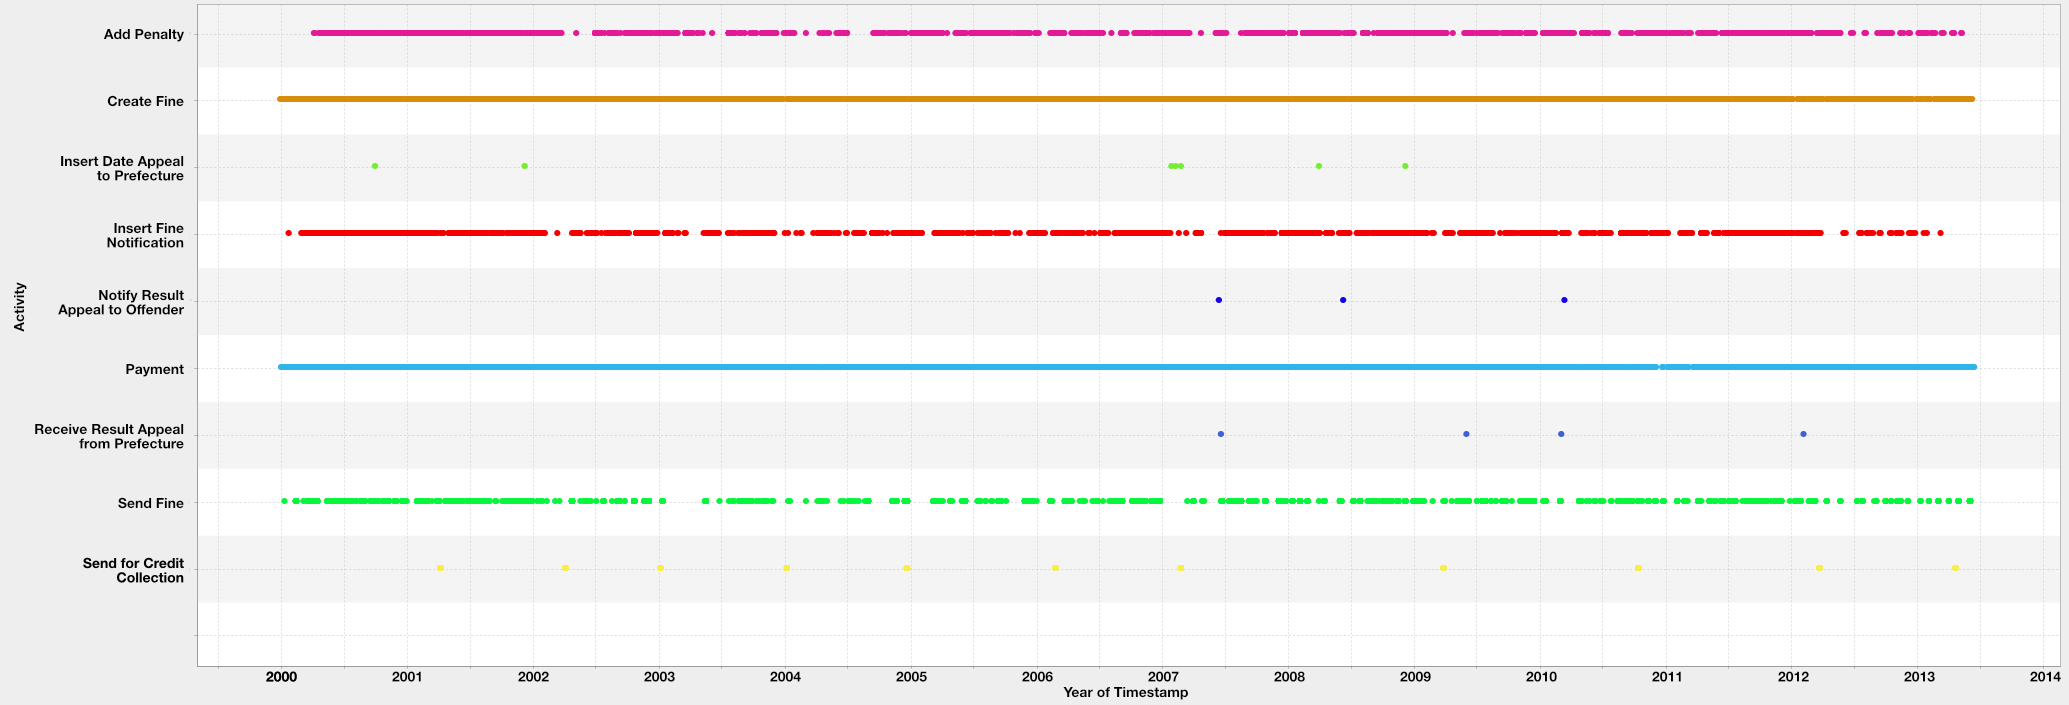
\includegraphics[width=\textwidth]{figures/dotted_timestamp.png}
  \caption{Event occurrences for cases without an appeal, grouped by activity type over time.}
  \label{fig:dotted_timestamp}
\end{figure}

The second chart that can be seen in figure \ref{fig:dotted_duration} also shows the different activity types on the y-axis. However the events are now plotted over the case duration at the time that the event occurred. This case duration metric was automatically computed by the used \emph{LogProjection} plugin. We see that \texttt{Create Fine} is always the first event of every case, as was already discovered in \textbf{c)}. The activity is therefore only observable at the beginning of the chart. \texttt{Send for Credit Collection} activity only starts after almost a full year of case duration and is the activity that is performed the latest in most cases. The first activity after one year can be explained with the findings from the previous chart, where it was discovered that the activity is only performed once a year. The \texttt{Payment} activity also has some events performed in late stages of the process instances, but is also frequent throughout all case durations. The other activities are mostly performed within the first year of an active case. The \texttt{Notify result Appeal to Offender} activity is always performed before the \texttt{Receive Result Appeal from Prefecture} activity. Overall we can see that the activities that are performed directly by the police department occur earlier in the cases or in cases that have an overall shorter duration. Activities that are depending on the offender and are related to payments appear at the very end of the case. The longest case durations are therefore caused by cases in which the offender makes a delayed payment. It is also visible that the frequent events are mostly spread across the whole range of case durations, with only a small reduction towards the extremely long case durations. This suggests that there are no peaks in case duration and there is an almost equal distribution of case durations over the timeframe.

\begin{figure}[H]
  \centering
  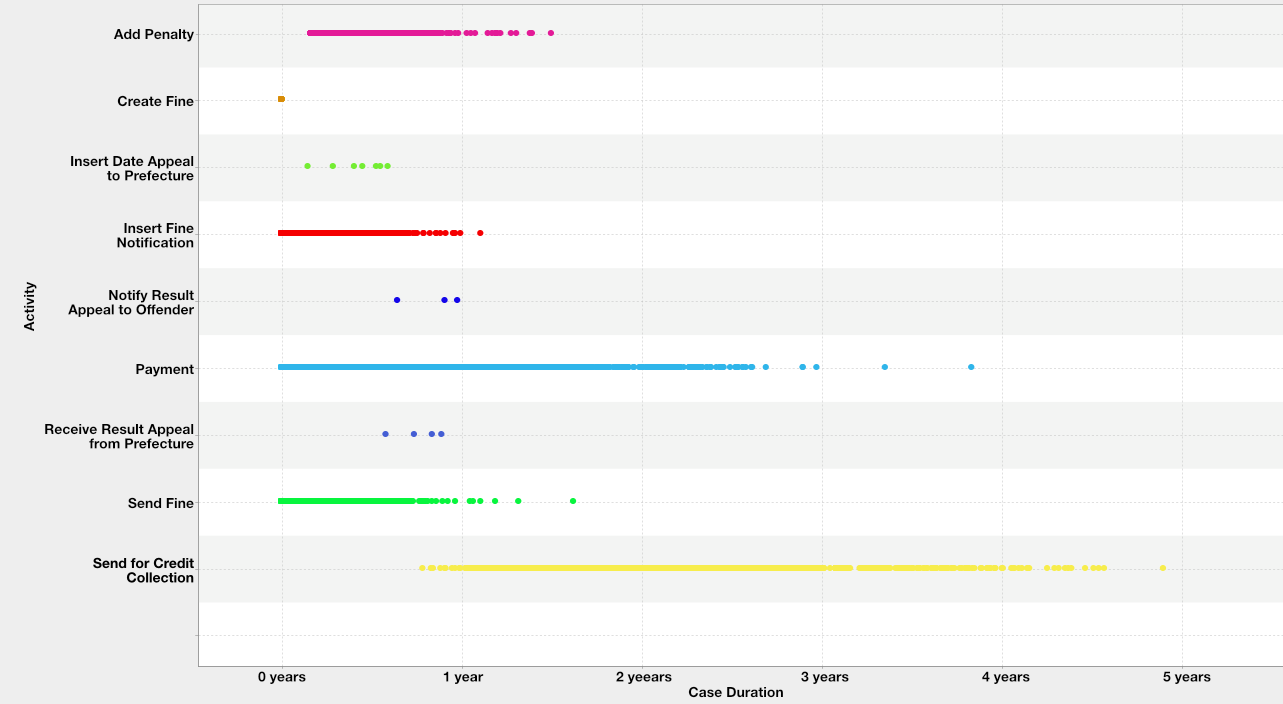
\includegraphics[width=\textwidth]{figures/dotted_duration.png}
  \caption{Event occurrences for cases without an appeal, grouped by activity type over the case duration at the time the event occurred.}
  \label{fig:dotted_duration}
\end{figure}

\paragraph{\textbf{e)}}


Since all lifecycle transitions are complete events the number of events and activities are equal. Furthermore, we computed the absolute and relative frequencies of the activities in each log.

\begin{table}[H]
\centering
\begin{tabular}{|l|l|l|l|l|}
\hline \textbf{Activity} & \textbf{Original} & \textbf{Appeals} & \textbf{No Appeals} \\
\hline Add penalty & 79860 & 4357 & 75503\\
\hline Appeal to Judge & 555 & 555 &0\\
\hline Create Fine & 150370 & 4513 & 145857\\
\hline Insert Date Appeal to Prefecture & 4188 & 4146 & 42\\
\hline Insert Fine Notification & 79860 & 4357 & 75503\\
\hline Notify Result Appeal to Offender & 896 & 863 & 33\\
\hline Payment  & 77601 & 903 & 76698\\
\hline Receive Result Appeal from Prefecture & 999 & 964 & 35\\
\hline Send Appeal to Prefecture  & 4141 & 4141 & 0\\
\hline Send Fine  & 103987 & 4513 & 99474\\
\hline Send for Credit Collection & 59013 & 412 & 58601\\
\hline
\end{tabular}
\caption{Absolute Frequencies of Activities in the Event Logs}
\label{tab:1c_absolut}
\end{table}

\begin{table}[H]
\centering
\begin{tabular}{|l|l|l|l|l|}
\hline \textbf{Activity} & \textbf{Original} & \textbf{Appeals} & \textbf{No Appeals} \\
\hline Add penalty & 0.142234 & 0.146582 & 0.141991\\
\hline Appeal to Judge & 0.000988 & 0.018672 &0\\
\hline Create Fine & 0.267815 & 0.151830 & 0.274298\\
\hline Insert Date Appeal to Prefecture & 0.007459 & 0.139483 & 0.000079\\
\hline Insert Fine Notification & 0.142234 & 0.146582 & 0.141991\\
\hline Notify Result Appeal to Offender & 0.001596 & 0.029034 & 0.000062\\
\hline Payment  & 0.138210 & 0.030379 & 0.144238\\
\hline Receive Result Appeal from Prefecture & 0.001779 & 0.032432 & 0.000066\\
\hline Send Appeal to Prefecture  & 0.007375 & 0.139315 & 0\\
\hline Send Fine  & 0.185205 & 0.151830 & 0.187071\\
\hline Send for Credit Collection & 0.105104 & 0.013861 & 0.110205\\
\hline
\end{tabular}
\caption{Relative Frequencies of Activities in the Event Logs}
\label{tab:1c_relative}
\end{table}

All traces of the original log begin with a 'Create Fine' activity. Therefore, the fraction of traces starting with 'Create Fine' is $1$ and $0$ for all other activities. Of course, this is also the case for both sub-logs. \\
The following activities are the only activities that occur as end activities of traces:

\begin{table}[H]
\centering
\begin{tabular}{|l|l|l|l|l|}
\hline \textbf{Activity} & \textbf{Original} & \textbf{Appeals} & \textbf{No Appeals} \\
\hline Payment  & 0.446904 & 0.154443 & 0.455953\\
\hline Send for Credit Collection & 0.392346 & 0.087747 & 0.401770\\
\hline Send Fine  & 0.138026 & 0.001551 & 0.142249\\
\hline Send Appeal to Prefecture  & 0.020908 & 0.696654 & 0\\
\hline Appeal to Judge & 0.000891 & 0.029692 &0\\
\hline Notify Result Appeal to Offender & 0.000572 & 0.018170 & 0.000027\\
\hline Receive Result Appeal from Prefecture & 0.000352 & 0.011744 & 0\\
\hline
\end{tabular}
\caption{Fraction of Traces that end with the Corresponding Activity}
\label{tab:1c_end}
\end{table}

Using Tabel \ref{tab:1b} we can compare the tree logs on a basic level. As expected, the majority of
cases do not contain a appeal event. Only around $3\%$ of traces have an appeal. But since the average trace length is
significantly longer in the cases with an appeal, the events in the log with appeals are around $5.3\%$ of the original log.
With 60 unique traces the log with traces is responsible for a disproportionately high trace variety. The original and the log
without appeals have data starting on the 01.01.2000 until the 18.06.2013. The timespan of the log with appeals is very similar
only starting a few days later and ending a few days earlier. This is to be expected due to the relatively low amount of traces
with an appeal. Interestingly, the log with appeals contains far less traces with duplicate activities than the other two logs. \\

Some interesting insights can be gained by looking at the absolute and relative frequencies of specific activities in Table \ref{tab:1c_absolut} and Table \ref{tab:1c_relative}.
First of all, we can note that there are no appearances of the activities 'Appeal to Judge' or 'Send Appeal to Prefecture' in the log without appeals.
There are still some activities that should only be in the log with appeals such as 'Notify Result Appeal to Offender' but these occurrences can
be considered noise and ignored. An open question that could point to a possible problem is the high amount of traces containing 'Send for Credit Collection' in the log without appeals. Especially, when keeping in mind that this activity is batched together. It is very likely that the average
case duration could be reduced if there were less cases where the fine has to be collected externally. The same thing can also be observed in Table \ref{tab:1c_end}. Furthermore, in the case without appeals, there are many traces ending with a 'Send Fine' event which points to a high number of unpaid fines. Further analysis should investigate if this suspicion is true and what can be done against it.

\section{Q2. Discovery and Conformance}

\section{Q3. Attribute Analysis and Compliance}

\section{Q4. Performance}

\section{Q5. Summary and Conclusion}

\section*{Appendix}

\end{document}

